\part{Introduction}
%Summary: DELETE THIS AFTERWARDS

%Gene regulation as a source for change: evolution and disease
%Evolution: the appearance of main morphological novelties, like paired structures, land conquest, and vertebrates. At this point talk about Amphi as a great model to understand these novelties.
%Also talk about how evolution is a continuous and we can use it to explain differences between very similar species like laevis and tropicalis. Even in the same species like the chromosome copies in laevis, cave traits, feather differences in the same species of birds and so. This points towards Astyanax as a model for understanding evolution, and also gene regulation at micro-evolutionary scale. 
%SQUEME:
%\begin{itemize}
%\item Gene regulation: Cis and trans regulation: Explain briefly (jaja) trans regulation and cis regulation. Here we will probably need some epigenetics explanations.
%\item Evolution: you need to relate gene regulation to evolution. Examples of these can be found in the gli3 paper, and Letelier paper. Co-options of GRN and this kind of things. Please dont go back to Darwin Ale. Once you have completed this, you need to introduce amphioxus as a model organism to understand vertebrate body plan and also you need to introduce some signalling pathways (this is where the fun begins).
%\item Evolution at micro-evolutionary scales. Here the link is more difficult, but you can explain that evolution is a continuous and gene regulation is a key player in such small distances. Use the ciclid fish speciation as example, also stickleback (this is a little trick for the discussion actually). ¿¿¿¿Then you move to the link of gene regulation to disease???? and finally you present the cavefish as a great model for studying microevolution.
%\end{itemize}

The diverse forms that life has adopted on our planet have been a source of marvel and study for humankind since ancient times. From this desire to understand life, the field of Biology emerged thousands of years ago. From the early classification methods of life that Aristotle developed to Carl Linnaeus's taxonomical system, in which modern taxonomy has its foundations, we have always tried to understand and classify the great variety of life based on its morphology. In these classification systems, humans are together with the rest of the animals, and we share common characteristics. With the development of molecular biology and modern taxonomy, this picture has emerged as a clear crystal to our eyes. Integrating different fields like genetics, evolutionary Biology, and Developmental Biology, the EvoDevo field has given us significant advances in how animal shapes evolve. 
During the duration of this thesis, we try to expand our knowledge of  how gene regulation has impacted the evolution of organisms. This question has been addressed several times, with more or less a degree of success, and here we present our approach to better understand this matter. But first of all, we need to understand with a reasonable depth how gene regulation operates in different organisms and how our work is relevant to the field. The next series of chapters and subchapters will try to guide the reader through this extensive and fascinating field of knowledge: gene regulation. Finally, we will discuss some already-known examples of how gene regulation affects the evolution of animals.


\chapter{Gene regulation during embryonic development}

Although multicellular organism cells share the same genetic information encoded in their DNA, the differential usage of this genetic library has allowed them to maintain and develop different tissues and organs. The central dogma of molecular biology is tightly regulated at its various levels to ensure that the different gene products are expressed in the right place and at the right time. These mechanisms allow different cell compositions in terms of gene products, making cells of different tissues differ in their protein content and composition. In other words, the cells control their gene expression in response to developmental and environmental cues. During embryonic development of multicellular organisms,  cells take regulatory decisions which will drive them to a specific cellular fate. In this process, a single cell, the zygote, bearing a single copy of its genome, will undergo gene regulation at different levels to form a complete organism. At early developmental stages, minimal deviations from the transcriptional program have severe consequences, from developmental defects to lethal phenotypes. Since these consequences can affect the successful reproduction of the organism, gene regulation is under heavy evolutionary pressure. This is why understanding the precision of gene regulation during development and through evolution is a key field of Evolutionary Developmental Biology.

Cells have several mechanisms to control their protein and gene product composition, or in other words, gene expression. One of the most important mechanisms to control gene expression takes place at the level of transcription. Transcriptional regulation is the process through which the amount of RNA molecules that will be transcribed from a specific gene locus is determined. Next, at the post-transcriptional level, these RNAs undergo modifications affecting their stability \parencite{boo_emerging_2020}. Moreover, alternative splicing is another regulatory step that determines which sequence of exons of the recently transcribed RNA molecule will be translated into the final gene product \parencite{marasco_physiology_2022}. Finally, there are additional regulatory mechanisms at the translational and post-translational level, as for example, the control of the translational efficiency of mature mRNA molecules \parencite{xue_rna_2015}. All these mechanisms control only one layer of the central molecular dogma, the RNA level. Notably, these complex regulatory layers of gene expression are conserved in animals and are also under tight regulation. These mechanisms alone cannot explain how transcriptional regulation takes place on a given set of specific genes. In the next sections, we will describe the mechanisms of transcriptional regulation, and what are the key players in this process.

\section{\textit{Cis} regulation of the genome}



The genome can be divided into coding and non-coding regions. The coding fraction, which comprises only 2\% of the genome in humans, contains the gene loci that will be transcribed and translated.  Until recently, this part of the genome received all the attention, whereas the non-coding part was overlooked. The ENCODE project was a critical milestone in understanding the regulatory function of the non-coding part of the genome \parencite{consortium_integrated_2012}. 


\textit{Cis}-regulatory elements (CREs) are non-coding regions of the genome that play a central role in gene transcription. These regions can recruit the transcription machinery and/or transcription factors (TFs) to fine-tune the gene expression. These CREs can affect the transcription in different manners. Enhancers and promoters will have a positive impact on the transcription of the target gene locus. Silencers and insulators, on the other hand, have a repressive role in transcription. Except for promoters, CREs can control the gene expression of the target genes with relative disregard for the genomic distance. We will briefly describe the role of promoters and enhancers in transcriptomic regulation since they are the most studied CREs.

Promoters are CREs in close spatial relationship with the gene they control, and in these regions is where the transcription of a gene starts. They are composed of two different regions, the core promoter and the proximal promoter. The core promoter of a gene is an approximately 80 base pair (bp) region that is centred in the Transcription Start Site (TSS) of the gene. The transcription machinery will bind to this region to prime transcription. This transcription machinery comprises RNA polymerase II and general TFs, which together form the Pre-Initiation Complex (PIC) \parencite{haberle_eukaryotic_2018}. Based on their characteristics, they can be divided into different types of core promoters \parencite{haberle_eukaryotic_2018}: the ones that regulate genes important for the terminal differentiation of cells, the ones of developmental genes, and the ones of housekeeping genes. The activity of the core promoter can be modulated by other TFs and cofactors, which will bind to a region upstream of the core promoter, the proximal promoter. This region contains sequences that will be recognized specifically by TFs, the TF binding sites (TFBS). The proximal promoter recruits itself TFs to modulate the transcription but can also interact with other genomic elements, like silencers or enhancers. This interaction is independent of the genomic distance and modulates the transcription depending on the combinations of TFs that are brought together. 


Enhancers are regions of the genome that promote the target gene's transcription by recruiting specific TFs and transcriptional coactivators. One single enhancer can have several target promoters, which can be thousands of kilobases (kb) away \parencite{tena_evolutionarily_2011}. The region where we can find the enhancers that regulate one gene is called the Regulatory Landscape (RL). Another property of enhancers is that they are modular. This means that the gene expression pattern of a gene is driven in different tissues by different tissue-specific enhancers. For example, the gene \textit{SHH} is expressed in several tissues, but a specific enhancer named ZRS drives the expression of this gene to the limbs \parencite{lettice_long-range_2003}. Nevertheless, although there are other examples of genes that owe their expression pattern to modular enhancers, there is increasing evidence that there are also pleiotropic enhancers. These enhancers can drive gene expression of different genes in different tissues \parencite{singh_enhancer_2021}. This characteristic is especially important for developmental genes since different enhancers control their spatiotemporal specificity. Developmental genes have a greater number of enhancers in their RL than other genes to precisely control the developmental gene expression \parencite{calle-mustienes_functional_2005}. The control of the gene expression of developmental genes tends to be robust thanks to the redundancy their enhancers provide \parencite{osterwalder_enhancer_2018, waymack_shadow_2020}. TFs that bind to enhancers have a well-defined spatiotemporal expression pattern in the organism. The regulatory information encoded by these TFs is integrated into the target gene's promoter. The specificity of transcription of the target gene is given by a certain combination of TFs. Enhancers can also have a repressive role in transcription, and these elements are often called silencers. In recent years it has been demonstrated that these elements are dual CREs; depending on the cellular context, they either enhance or repress transcription \parencite{santos-pereira_pioneer_2019, gisselbrecht_transcriptional_2020, segert_transcriptional_2021}.

The interaction between enhancers and promoters is not always easy to discern. One enhancer can interact with a promoter located several kilobases away, regardless of other promoters that lie in between. The specificity of the interaction between enhancers and promoters is currently being investigated by several groups, while several conclusions have been drawn in recent years \parencite{pachano_enhancer-gene_2022}. First, there are genes with different classes of promoters, which vary in their capacity to integrate regulatory information. Housekeeping promoters are not responsive to distant enhancers because the regulatory information they integrate is very close to their promoters or even encoded in themselves \parencite{zabidi_enhancercore-promoter_2015}. These promoters tend to have a broad distribution of TSSs that is accompanied by unmethylated CpG islands. Other promoters, the promoters of tissue-specific genes expressed in terminally differentiated cells, only integrate information from nearby enhancers and tend to have a sharp distribution of TSSs. And finally, developmental gene promoters are regulated by distal enhancers and tend to have a broad distribution of TSS and unmethylated CpG islands, which can extend even to the body of the gene. 

Enhancers can find their target gene promoter regardless of their linear genomic distance thanks to the tridimensional (3D) folding of the chromatin, which facilitates their close interaction. The 3D organization of the genome makes it possible for meters of chromatin to be folded in the nucleus of the cell in an ordered way. This 3D structuring of the genome has different layers of organization. In one of the first layers, there are some specific CREs, called insulators, that interfere with enhancer-promoter interactions, separating the regulatory landscapes of genes. Insulators help to segment the genome in structural units known as topologically associated domains (TADs). Insulators are the platform where architectural proteins and TFs bind in the genome, like \textit{CTCF}. These structural proteins are crucial during development to generate the 3D folding of the genome and to maintain the specificity of enhancer-promoter interaction \parencite{arzate-mejia_developing_2018, franke_ctcf_2021}. 

The different classes of CREs play different roles in organizing gene regulation, and understanding how they work is critical for knowing the mechanisms of development and disease in animals.The study of these elements and their interplay in transcriptional regulation has greatly benefited from the emergence of Next Generation Sequencing (NGS) techniques. For example, RNA-seq allows us to study the total transcriptional output of an organism, a tissue, or even a single cell \parencite{wang_rna-seq_2009, sebe-pedros_cnidarian_2018, geirsdottir_cross-species_2019, farnsworth_single-cell_2020, gao_long_2022}. Not only the transcriptional output, but also the regulatory regions and how they interact with their target gene in the 3D space of the nucleus have been described in recent years. The decrease in cost and input material has enabled the use of these techniques in different organisms. These techniques have allowed for the identification of conserved non-coding elements and cis-regulatory modules that control gene expression during development, which has helped to uncover the underlying genetic mechanisms of development. This has provided new insights into the evolution of gene regulation and the mechanisms by which new traits and body structures arise. Understanding how epigenetic mechanisms impact the transcriptional readout is critical for understanding animal development and evolution.



\section{Epigenetics and tools for its study}


The DNA in eukaryotes is compacted in the nucleus of the cell. The first level of DNA packaging is chromatin, a combination of DNA with histones. The structural units of the chromatin are the nucleosomes, comprised of 147 bp of DNA and an octamer of histone proteins. There are mechanisms that alter these structural units and change the gene expression without modifying the DNA sequence. In fact, chromatin remodelling and methylation are epigenetic mechanisms that are of key importance for gene regulation \parencite{margueron_chromatin_2010, bonasio_molecular_2010, ashe_how_2021}. Using various NGS techniques and thus assessing chromatin accessibility, histone marks and DNA methylation, we can infer different chromatin states. These must be tightly regulated to achieve precise spatiotemporal gene expression patterns for normal development and physiology. In fact, epigenomic mechanisms allow multicellular organisms to develop and function using the same DNA information in all their cells. 

When a CRE is active, the region where TFs are bound is depleted of nucleosomes, leaving the chromatin accessible \parencite{brahma_epigenome_2020}. There are some TFs, known as pioneer TFs, that have the ability to bind to closed chromatin, triggering its opening and modifying its state to active \parencite{larson_pioneering_2021, balsalobre_pioneer_2022}. These accessibility changes alter the binding of TFs to chromatin, which is crucial for embryonic development. Their ability to bind to specific CREs in the genome allows them to regulate the expression of target genes, controlling cell fate specification, migration, morphogenesis, and differentiation. Several NGS techniques have been developed based on the opening of the chromatin to infer CRE activity, like DNase-seq \parencite{boyle_high-resolution_2008, hesselberth_global_2009, song_dnase-seq_2010}, MNase-seq \parencite{yuan_genome-scale_2005}, and ATAC-seq \parencite{buenrostro_transposition_2013}. In the latter, we employ the bacterial transposase Tn5, which preferably access and cut DNA that is not associated with nucleosomes. A modified transposase can simultaneously fragment the DNA and add NGS sequences bearing barcodes at the edges of the cleaved regions. The results of these techniques constitute a proxy to detect potential CREs, and subsequently which TFs are bound onto them \parencite{bentsen_atac-seq_2020}. However, there are some limitations concerning these techniques. For example, they are not useful to distinguish different classes of CREs, since relaxed chromatin is a mark for activity of all of them. In order to know which type of CRE we detected, we need to use other techniques that assess the epigenomic state of the nucleosomes flanking these open chromatin regions.


Histones composing nucleosomes undergo post-translational modifications in their amino acid tails that constitute key epigenetic marks. These epigenetic modifications condition the binding of regulatory proteins to the histones. Histone modifications include acetylation, methylation, phosphorylation, and ubiquitination. Histone acetylation is typically associated with active chromatin and the increased accessibility of DNA to the transcription machinery. One of the most common acetylation marks is H3K27Ac, associated with active enhancer regions and important in regulating transcriptional activation. On the other hand, histone methylation has an activatory or repressor effect on gene expression, depending on the amino acid residue \parencite{barski_high-resolution_2007}. One of the most common methylation marks is H3K27me3, which is associated with the repression of gene expression and is found in regions such as Polycomb repressed elements \parencite{guo_polycomb_2021}. In contrast, H3K4me3 is a mark associated with active promoters and is fundamental for gene expression activation. The combinatorial effect of multiple histone modifications results in different chromatin states \parencite{rada-iglesias_unique_2011, haberle_eukaryotic_2018}. For example, the presence of both H3K4me3 and H3K27Ac marks in the same chromatin region and chromatin relaxation indicates that this region is an active promoter, while H3K4me1 and H3K27ac hint towards an enhancer element. This combinatorial effect allows for more complex gene expression regulation and dynamic responses to physiological and environmental cues. Different chromatin states affect the capacity of TFs and coactivators to bind to CREs. To study the genome-wide binding of TFs and different histone modifications, Chromatin Immunoprecipitation followed by sequencing (ChIP-seq) is widely used \parencite{johnson_genome-wide_2007, massie_chromatin_2009, kaufmann_chromatin_2010}. This technique starts by chemically fixating the interaction between proteins and DNA, and subsequently fragmenting the chromatin. The fragments that are bound to the protein of interest are selected using a specific antibody, and they are sequenced using NGS techniques. This technique allows the assessment of the binding profile of TFs or modified histones. As such, we can assess where these proteins of interest bind on the genome. The analysis of binding sites of several TFs (TFBS) has revealed that TFs have sequence preferences, which can be derived from ChIP-seq data and "stored" in Position Weight Matrices (PWMs). Together, ChIP-seq and PWMs make it possible to understand where TFs are binding to the genome and to determine the chromatin state in a given condition \parencite{stormo_determining_2010, aerts_chapter_2012}.

Another epigenetic readout of the chromatin state is the methylation of CpG islands. In general, methylation of the cytosine of CpG islands represses transcription \parencite{greenberg_diverse_2019} by impairing the binding of TFs to the methylated enhancer or promoter. The control of methylation and demethylation of CpG islands located in enhancers and promoters is crucial for development since it allows the fine control of gene expression. For example, this tight regulation of methylation is required for specifying and maintaining the vertebrate germline \parencite{bogdanovic_dna_2017, bogdanovic_dynamics_2012, bogdanovic_active_2016}. The methylation of the genome can be explored using MethylC-seq, an NGS technique that uses bisulfite conversion of unmethylated cytosines to uracils to extrapolate CpG methylation.\parencite{bogdanovic_dna_2017}. Together with the previously mentioned techniques, this tool allows us to understand the regulatory logic behind determined conditions and stages. This regulatory logic is built on complex relationships between TFs, chromatin state and accessible CREs and their target genes. Studying these relationships is key to understanding the complexity of transcriptional programs deployed during the different stages of development. 




\section{Gene regulatory networks}

In the previous sections, we reviewed how CREs operate and the mechanisms that control CRE accessibility and TF binding. These mechanisms tightly control gene expression and have been conserved along the Tree of life. In developing embryos, these mechanisms determine the response of cells to their environment and the fate they will take on. Studying the sum of these responses is not trivial, since many TFs, 1659 TFs annotated in humans \parencite{shen_animaltfdb_2023}, are able to bind to several CREs in the genome. In fact, at a specific developmental time and tissue, there are a number of TFs, and signalling molecules expressed that bind onto specific CREs, which activate target genes. Target genes can be TFs themselves, regulating other genes. The combinations of those key elements and their interactions acting during development are represented by maps, known as Gene Regulatory Networks (GRNs) (Figure \ref{fig:Intro_grn_structure}). These interactions can be either activatory or inhibitory, visualized as lines connecting nodes which represent the genes  \parencite{levine_gene_2005}. 

The first characteristic of GRNs is that they are modular since they can be divided into functional sub-circuits. The second main characteristic of GRNs is that these sub-circuits are organized hierarchically, meaning that the activation of one circuit precedes the next one \parencite{davidson_gene_2006, wagner_developmental_2007}. On top of the hierarchy of GRNs, we have the core modules or kernels. These modules are composed of a series of TFs that will determine the cell fate of cell populations by interacting with several downstream regulatory circuits. TFs and their interactions present in kernels are under great selective pressure because of their high position within the GRN hierarchy. Kernel TFs tend to have plenty of interactions between them, forming feedback loops that secure the deployment of the kernel transcriptional program. We can find kernels that are conserved along great evolutionary distances, like the heart kernel \parencite{wijesena_antagonistic_2017} or the teeth kernel of vertebrates \parencite{sadier_role_2020}. Under the kernels, we find the secondary sub-modules. These circuits provide positional and temporal information since they integrate information from different signalling pathways. In these circuits, morphogens and the cellular receptors for these molecules provide positional information. The secondary sub-circuits can have several functions within a GRN. They can activate or repress kernels of other GRNs, or the effector genes, the last layer in the hierarchy of GRNs. The organization of the GRNs allows us to explore the relationship between these elements, structuring our knowledge about them and helping us to predict transcriptional outcomes. 

\begin{figure}[ht]
\centering
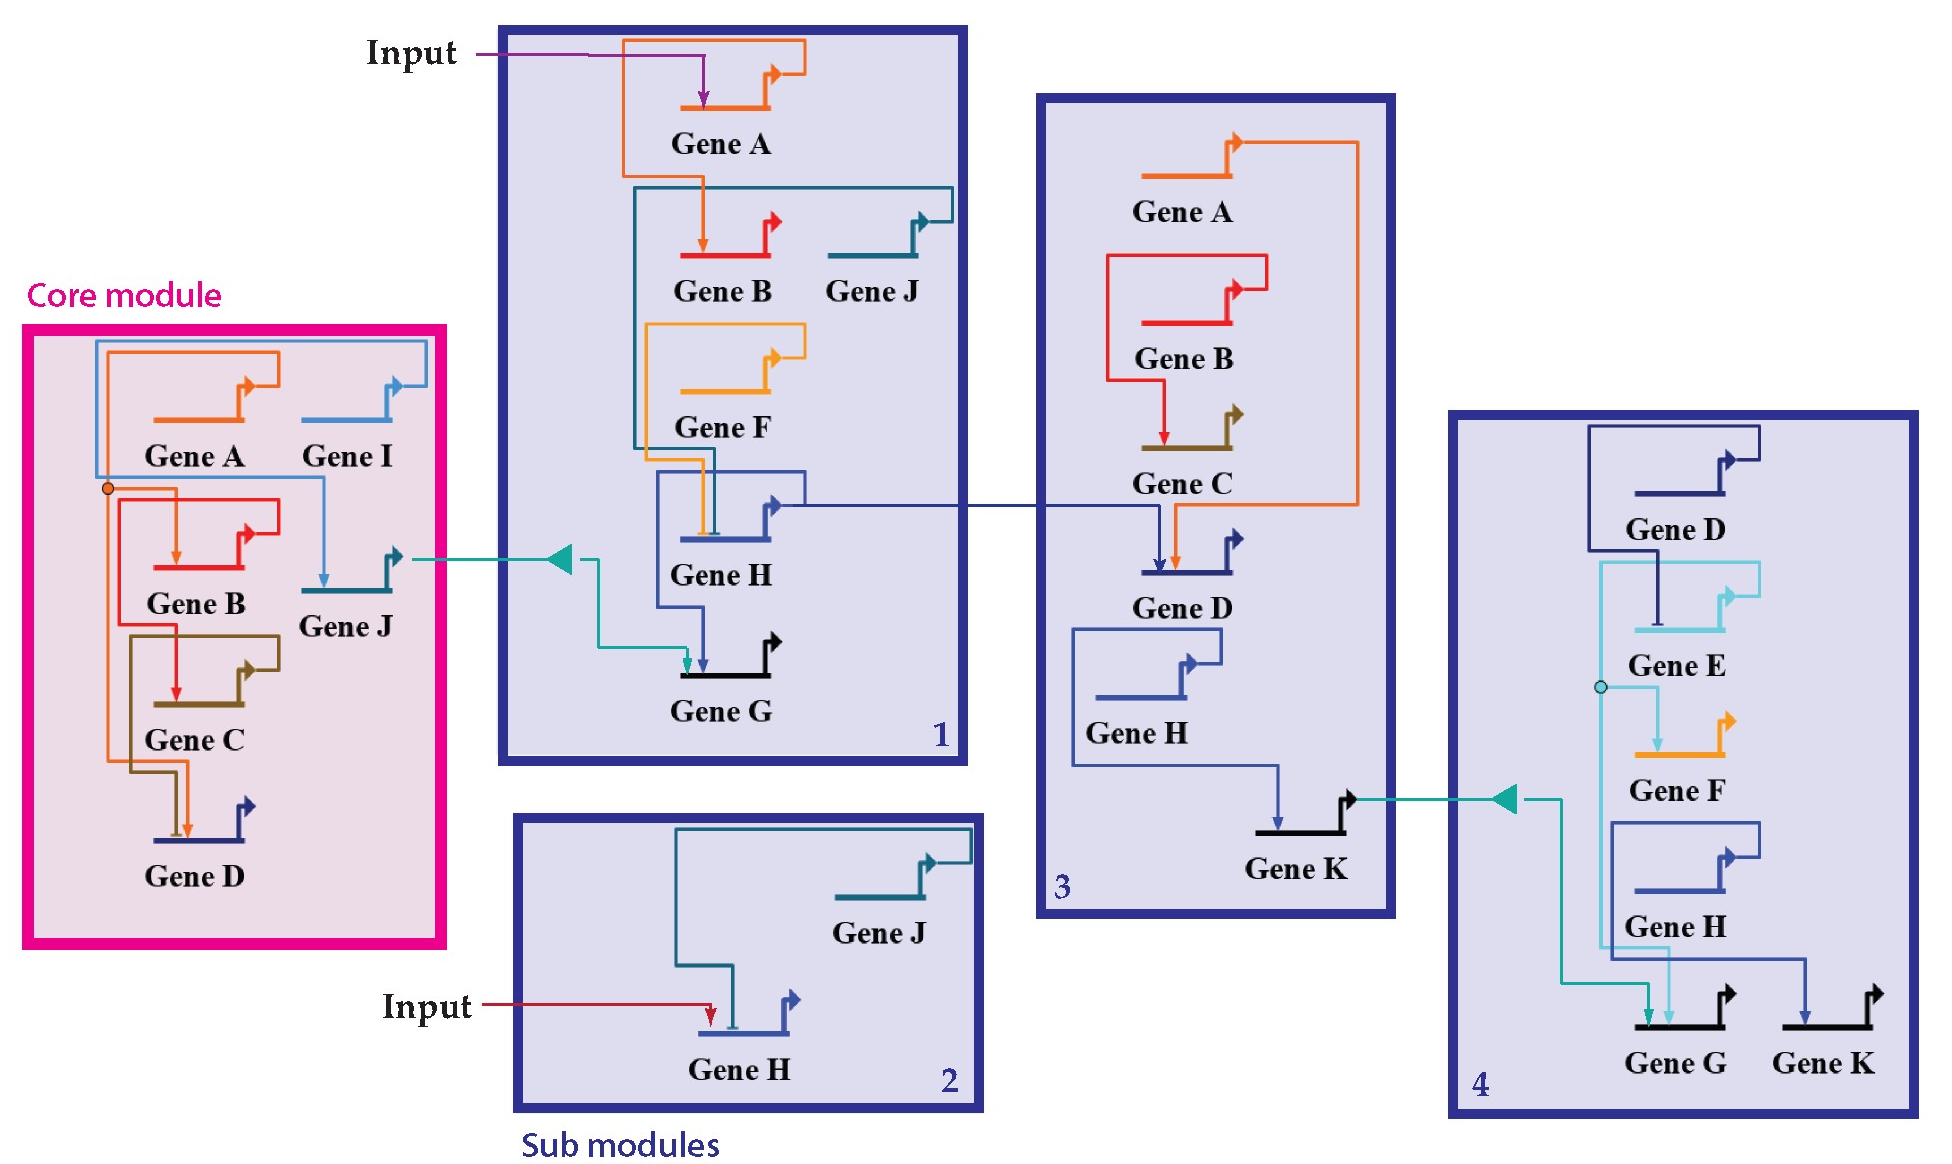
\includegraphics[width=1\textwidth]{Figures/Intro/GRN_structure}
\caption[GRN structure]{ Theoretical GRN structure. The GRN is divided into different sub-circuits, which are organized hierarchically, being the core module at the top of the hierarchy. Some genes, like Gene D, play a role in different sub-circuits, being part of different regulatory loops. Figure modified from \parencite{sadier_role_2020}}
\label{fig:Intro_grn_structure}
\end{figure} 


\section{Signalling pathways}

During development, cells respond to changes in the environment and the morphogens, giving rise to a viable embryo. This information is integrated into GRNs by common cell signalling pathways. Signalling pathways normally comprise a diffusible morphogen and a cellular receptor on which the morphogen binds, thus triggering a downstream cellular response. The gradient of morphogen concentration provides positional information to GRNs that will initiate a certain transcriptional program by activating GRN submodules. The modularity of these circuits makes possible the integration of this signalling information in the same GRN but at different hierarchical levels. For example, the genetic network controlled by \textit{Shh} is a fundamental signalling pathway in limb formation, but also for digit formation since it defines their number and position on the anteroposterior axis of the limb \parencite{lopez-rios_many_2016}. In the example of Figure \ref{fig:Intro_grn_structure}, we can observe that some genes, like Gene H, receive external inputs and are implicated in several secondary submodules of the GRN. These inputs are readouts of morphogen concentration of the developmental signalling pathway, and since the effector gene is in different submodules, the effect on the pathway will be different. Since several submodules respond to them, signalling pathways control a significant number of GRNs in development \parencite{pires-dasilva_evolution_2003}. The effector TFs of signalling pathways are usually integrated into several GRNs because they integrate several genetic cascades. Due to their high impact on animal development, signalling pathways have been highly conserved during metazoan evolution \parencite{babonis_phylogenetic_2017}.

One of the most conserved genetic networks in animals is the Wnt signalling pathway (Figure \ref{fig:Intro_wnt}). This signalling pathway is crucial in many different processes during embryonic development and in many cellular processes \parencite{steinhart_wnt_2018}. In the canonical Wnt pathway, when Wnt is not binding Frizzled, the pathway is inactive. In this scenario, inside the cell, the destruction complex will mark the main transductor of the signalling pathway, $\beta$-catenin, for ubiquitination, driving its degradation in the proteasome. When Wnt binds to the receptor complex Frizzled and LRP, Dishevelled (Dsh) is recruited. This protein will inactivate the $\beta$-catenin destruction complex, therefore increasing its intracytosolic concentration. $\beta$-catenin is then translocated to the nucleus, where it binds Lef/Tcf TFs and regulates the transcription of target genes. During development, Wnt concentration gradients are fundamental to establishing axial polarization in the dorsoventral and anteroposterior axes \parencite{niehrs_growth_2010, green_vertebrate_2015, genikhovich_evolution_2017}. In later stages of development, the Wnt signalling pathway is crucial in forming several organs, like limbs, skeletal muscles or the neural system, among others \parencite{brafman_wnt-catenin_2017, bertrand_developmental_2017, teufel_chapter_2019}. 




\begin{figure}[h!]
\centering
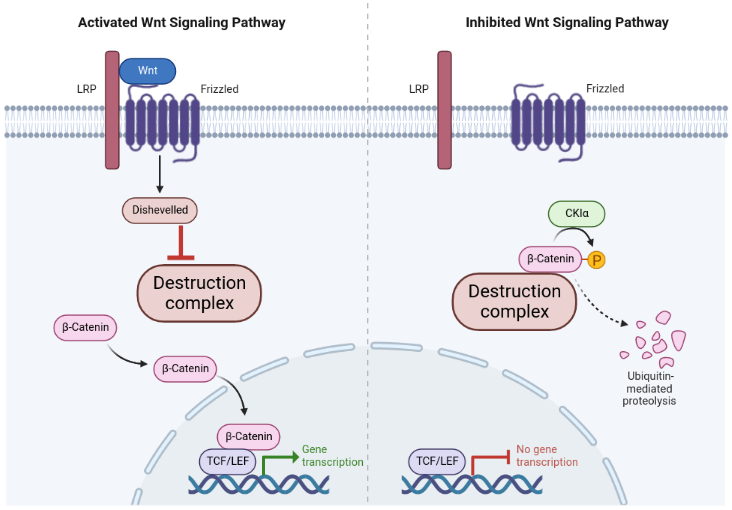
\includegraphics[width=1\textwidth]{Figures/Intro/Wnt_signalling.png}
\caption[Wnt pathway]{ Simplified view of how canonical Wnt signalling pathway is activated. When the Wnt ligand binds to the receptor Frizzled and the coreceptor LRP, the signal is transduced to the cytosol of the cell by Disheveled proteins, inactivating the destruction complex that degrades $\beta$-catenin. The concentration of $\beta$-catenin in the cytosol starts to rise, and the molecules are translocated to the nucleus, where it will bind TCF/LEF to activate target genes transcription. When the pathway is inactive, the destruction complex marks $\beta$-catenin for its degradation, impeding the translocation of $\beta$-catenin to the nucleus. Figure created using BioRender.}
\label{fig:Intro_wnt}
\end{figure} 

Similarly important for controlling several developmental processes in vertebrates is the retinoic acid (RA) pathway (Figure \ref{fig:Intro_RA}). When the cell receives the RA, it can trespass the cellular membrane and diffuse to the nucleus, where it binds the receptors of RA (RAR and RXR). These receptors form heterodimers and are bound to RA-responding elements (RARE). The combination of RA and its receptors triggers the transcription of target genes with RARE in their CREs like Hox genes \parencite{cunningham_mechanisms_2015, ghyselinck_retinoic_2019}. In its inactive form, the nuclear receptors of the RA can not initiate the transcription of the target genes. This signalling pathway is essential in  the patterning and development of several organs like the optic cup \parencite{bohnsack_zebrafish_2012}, heart \parencite{keegan_retinoic_2005} and hindbrain \parencite{abu-abed_retinoic_2001}.


\begin{figure}[h!]
\centering
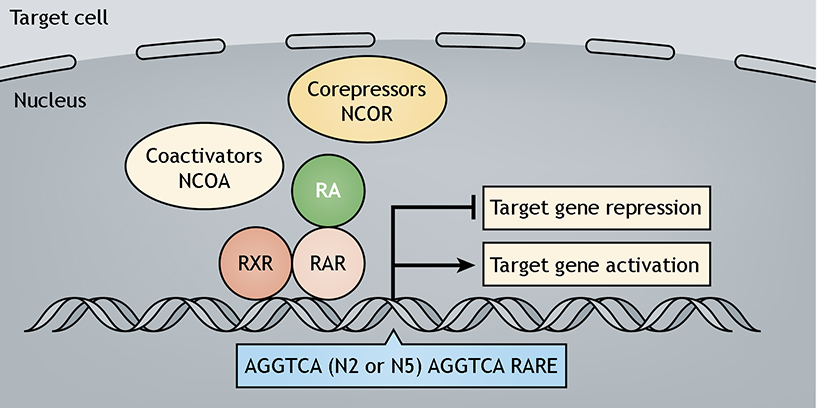
\includegraphics[width=1\textwidth]{Figures/Intro/Intro_RA.png}
\caption[Ra pathway]{RA can trespass the cellular membrane and diffuse directly to the nucleus. It binds its receptors (RAR and RXR), which are bound to the DNA in RA-responding elements. Depending on the conformation of RAR, this complex can recruit co-activators or co-repressors, controlling the transcription of target genes. Modified from \parencite{ghyselinck_retinoic_2019}.}
\label{fig:Intro_RA}
\end{figure} 

The fibroblast growing factor (FGF) signalling pathway is well conserved in animals and plays several roles during development \parencite{dorey_fgf_2010, babonis_phylogenetic_2017} (Figure \ref{fig:Intro_FGF}). This pathway is closely related to RA, and their regulatory antagonism makes possible the patterning of several structures during development \parencite{cunningham_mechanisms_2015}. The receptors of FGF, FGFR, are tyrosine-kinase proteins that dimerize when they bind FGF ligands. Once dimerized, the receptor units start a transphosphorylation between them that leads to the recruitment and activation of downstream pathways (RAS, PI3K, STAT, and PLC). During embryonic development, this pathway controls somitogenesis in coordination with RA \parencite{cunningham_mechanisms_2015} and the formation of several organs like the heart and limbs.

\begin{figure}[ht!]
\centering
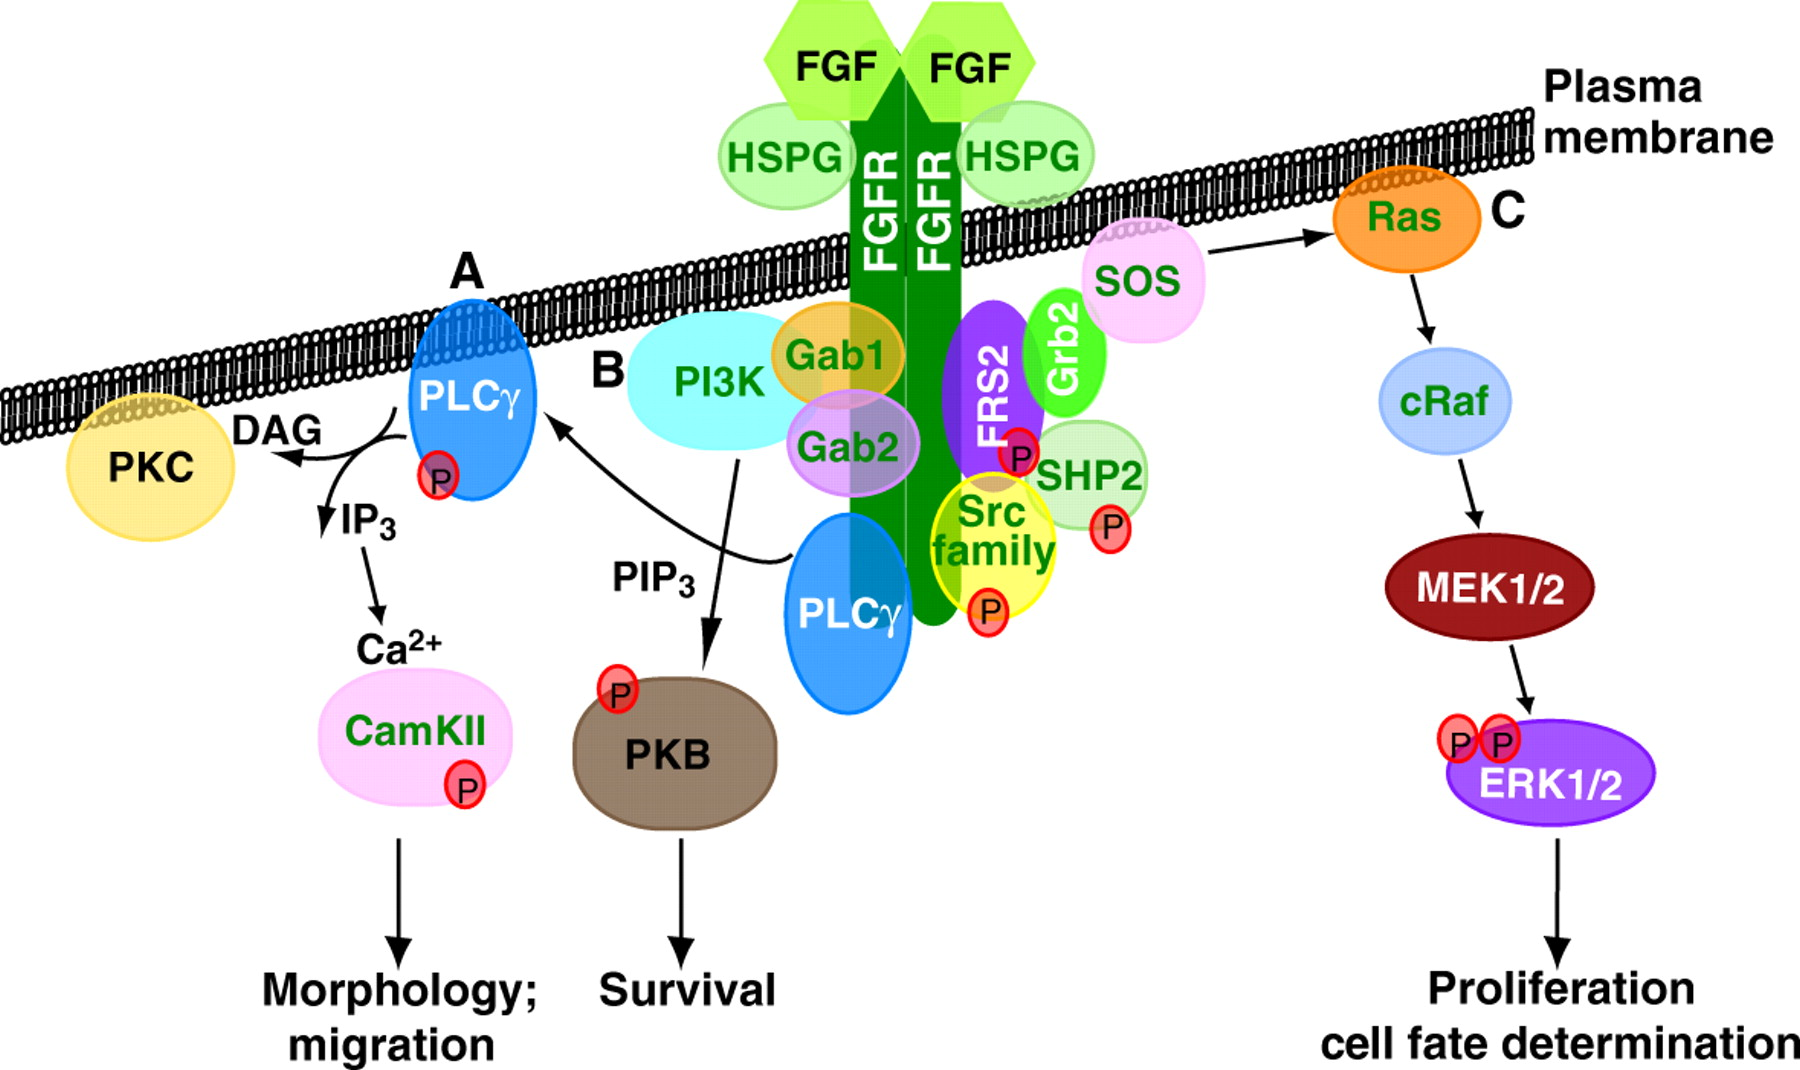
\includegraphics[width=1\textwidth]{Figures/Intro/Intro_FGF.jpeg}
\caption[FGF pathway]{When FGF ligands bind the FGF receptors (FGFR), this tyrosine kinase receptor transphosphorylates itself and recruits proteins that will transduce the signalling. These proteins are part of intracellular transduction pathways, like PLC, PI3K, RAS and STAT. This recruitment of transduction pathways will result in different transcriptional responses in target genes. Modified from \parencite{dorey_fgf_2010}}
\label{fig:Intro_FGF}
\end{figure} 


In close cooperation with the previous signalling pathways, TGF$\beta$ controls several processes during development \parencite{jia_tgf_2021} (Figure \ref{fig:Intro_Nodal}). Depending on which transduction mechanisms are used, TGF$\beta$ can be categorized into different families, being TGF$\beta$/ Nodal/ activin and BMP. TGF$\beta$/ Nodal/ activin ligands act as dimers and bind to the extracellular domain of type I and II receptors, forming a complex, sometimes together with a co-receptor. This complex will recruit effector proteins that bind to the cytosolic part of the complex and activate them by phosphorylation. These effector proteins are Smad2 and Smad3, and they form a heterotrimer with Smad4. The heterotrimer is then translocated to the nucleus to regulate the transcription of target genes in cooperation with other TFs. This signalling pathway is essential to determine the mesendoderm in vertebrate embryos \parencite{montague_vg1-nodal_2017}, to establish left-right asymmetry \parencite{hamada_diversity_2020} or patterning neural development \parencite{shen_nodal_2007}.

\begin{figure}[ht!]
\centering
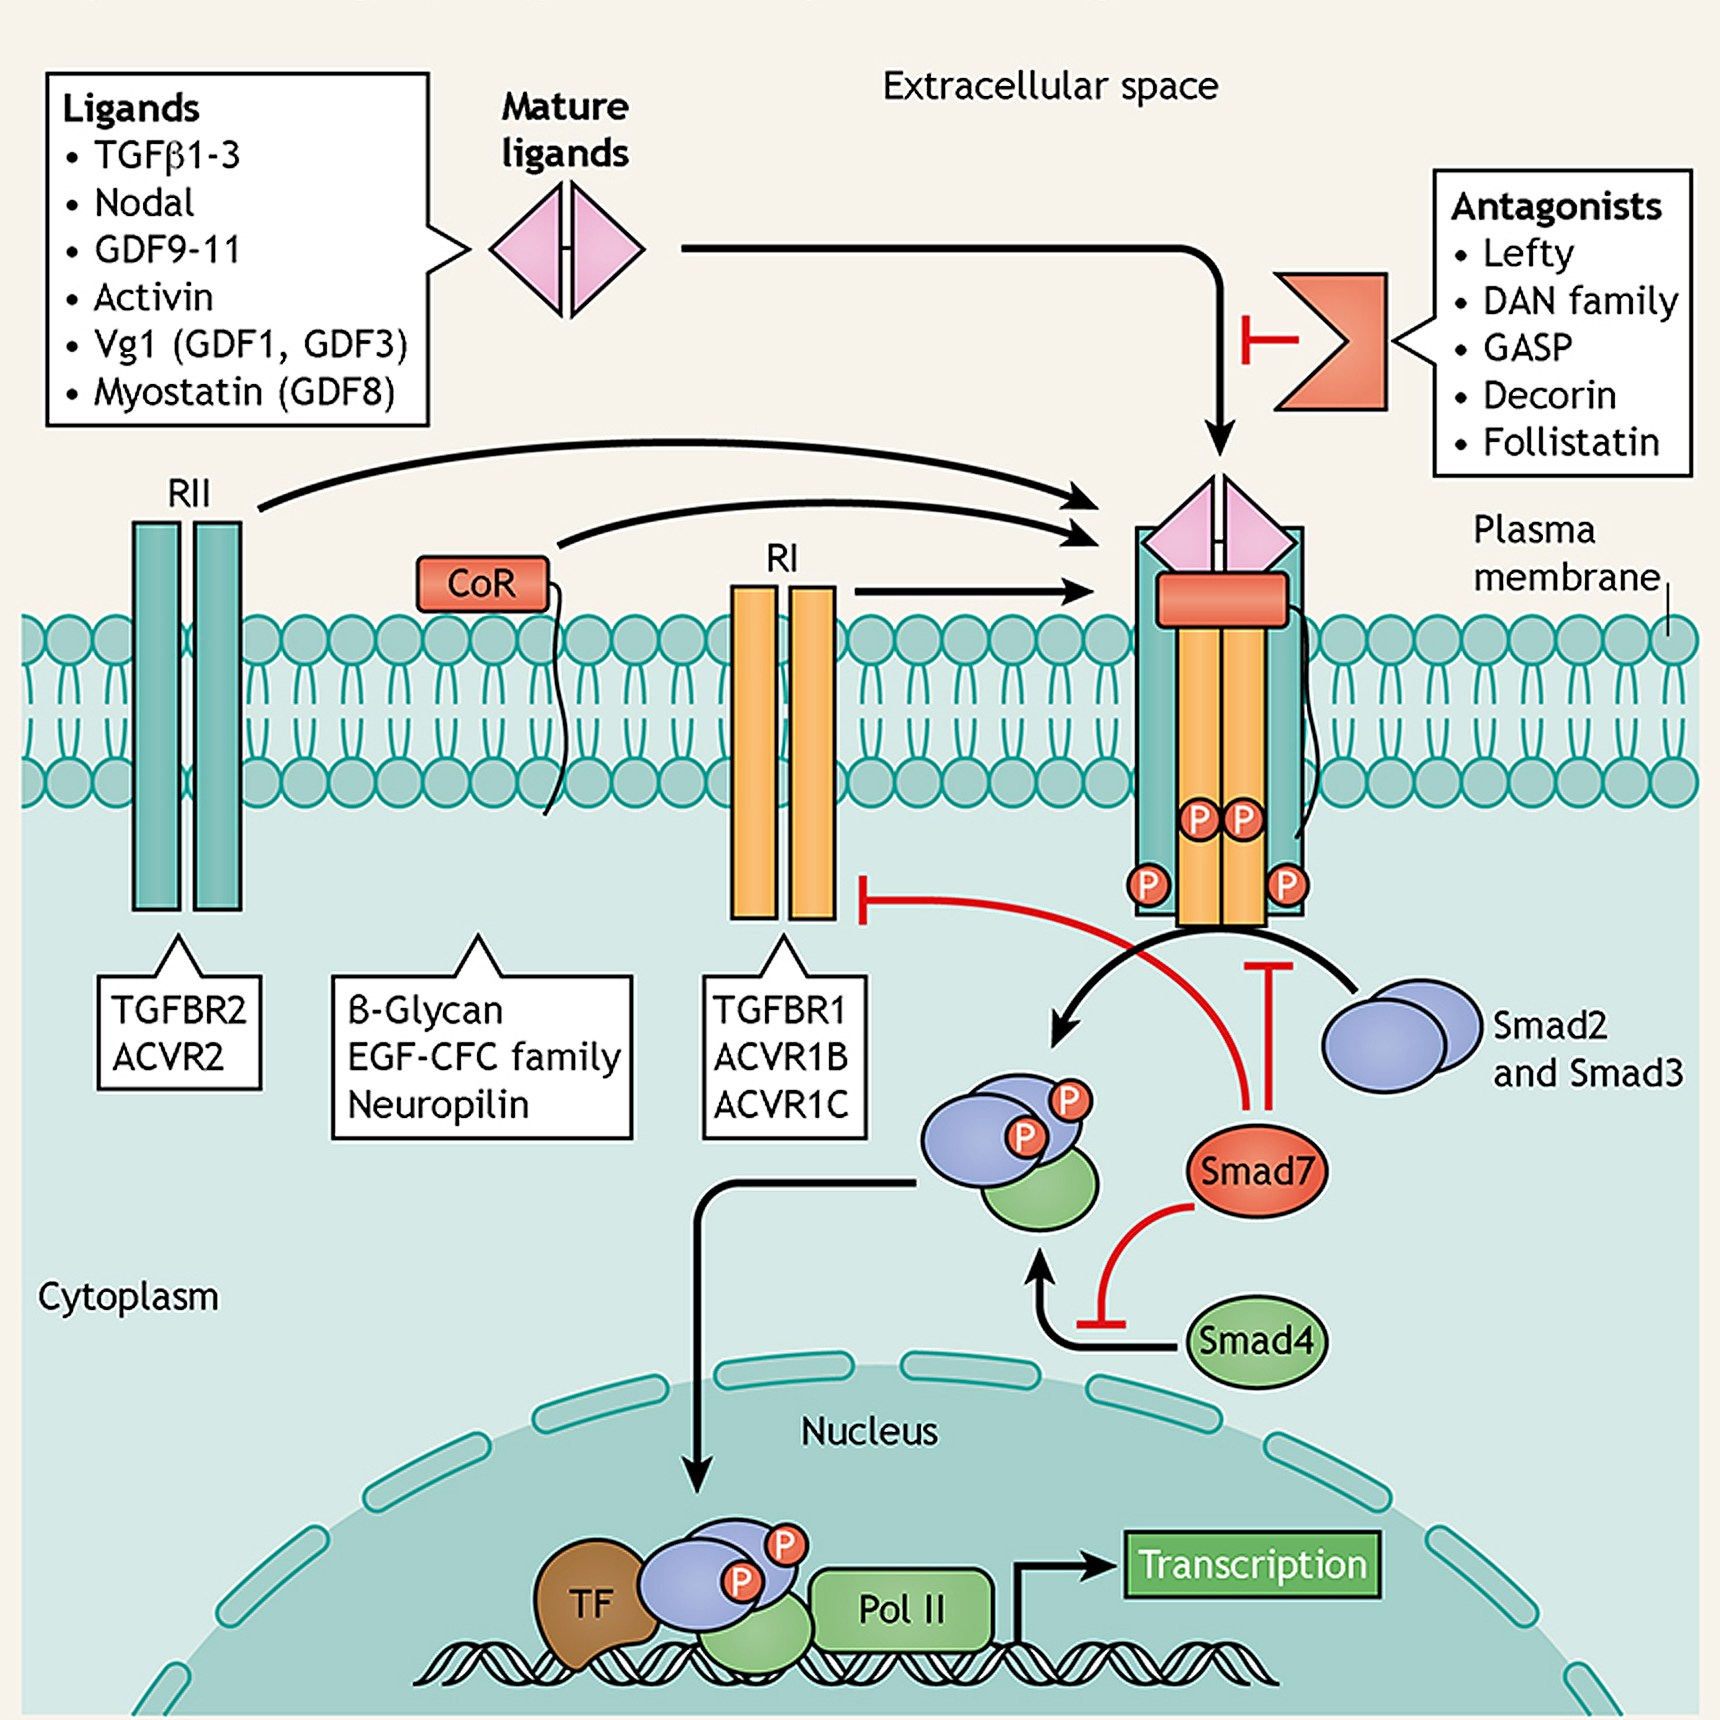
\includegraphics[width=1\textwidth]{Figures/Intro/Intro_Nodal.png}
\caption[Nodal pathway]{Nodal ligands bind to type I and II receptors (RI and RII), which form a protein complex in the plasma membrane. This complex, which includes sometimes the presence of a co-receptor (CoR), phosphorylates the effector proteins Smad2 and Smad4. Once activated, these factors form a heterotrimer together with Smad4 that is translocated to the nucleus to control the transcription of target genes, in close cooperation with other TFs. Modified from \parencite{jia_tgf_2021}. }
\label{fig:Intro_Nodal}
\end{figure} 


Developmental pathways operate in an interconnected manner. They control several GRNs, which can integrate information from several of these signalling pathways simultaneously. One example of this cooperation is the RA-FGF antagonism, which is critical for proper embryonic development. RA antagonizes the FGF pathway by inhibiting the transcription of FGF ligand proteins. \textit{Fgf8} gene in amniotes has a RARE in a -nearby-to-the-gene- enhancer that represses its transcription by recruiting co-repressors in a ligand-dependent manner \parencite{kumar_nuclear_2016}. GRNs provide the means to integrate this information and deploy different transcriptional programs accordingly. This integration is done at the TF level because they are the effector genes of signalling pathways and also an elemental unit of GRNs. Understanding the relationship between TFs and signalling pathways during development can provide insights into the mechanisms that control gene expression and cellular behaviour. It can also provide a better understanding of the causes of developmental disorders and malformations that result from defects in signalling pathways or TFs expression \parencite{weidemuller_transcription_2021}. Additionally, these signalling pathways are conserved along the evolutionary tree of animals and are critical to establishing the animal body plan. Moreover, little is known of how these signalling pathways are integrated in different animals, and what impact has this in gene regulatory complexity. Understanding the interactions between signalling pathways and GRNs and how they operate in different animals can give us insight into how the diverse morphology of animals has emerged during evolution.


\chapter{Gene regulation and evolution}

The emergence and diversification of different animal morphologies have been interesting fields of study for centuries. Darwin developed his theory on how natural selection has shaped this diversification of animal morphologies and made the scientific community aware of its importance \parencite{darwin_origin_1859}. He proposed that morphological diversity comes from random variations in populations and that these variations undergo a phenomenon known as natural selection. Natural selection depends on how the variations affect the fitness of the organism in a determined environment. The question of how these variations are acquired and inherited in the population arose. Almost 50 years after Darwin published his work, Morgan found the link between phenotypic changes and mutations in the DNA \parencite{morgan_sex-linked_1916}. His work helped bring together Mendelian inheritance and the changes in DNA affecting the phenotype. Later on, the discovery of the central dogma of molecular biology established a clear relationship between genotype and phenotype. At this point, developmental biology started to have a relevant weight in evolutionary biology, giving rise to what we call shortly as EvoDevo (Evolutionary Developmental Biology). 
EvoDevo tries to address how changes in genetic and molecular mechanisms of development affect the appearance and evolution of traits. One of the first breakthroughs in this field was the discovery of homeotic mutations. Ed Lewis and colleagues, while studying  \textit{Drosophila melanogaster}, found some unusual phenotypes. The flies that carried homeotic mutations had the identity of their body segments altered. Because of the change in the identity of body segments, the appendages associated with those segments were also changed. For example, instead of antennae, some mutants had legs since the head segment had changed its identity. In other cases, the identity of the abdomen was changed to a thorax, and those flies developed two pairs of wings \parencite{lewis_gene_1978}. Further studies revealed that only a few genes were responsible for these phenotypes. The discovery of these genes, known as homeotic genes, was a great landmark in EvoDevo since they control the identity of body segments not only in \textit{Drosophila melanogaster} but also in other animals \parencite{duboule_structural_1989, gehring_homeotic_1985, mcginnis_homeobox_1992, hueber_improving_2010, krumlauf_hox_2018}. The most important group of homeotic genes are the Hox genes, which are a set of homeobox genes that act as master regulators of developmental transcriptional programs since they control the segmentation of the body. Another striking characteristic of these genes is that they cluster together in the genome, and the expression pattern of these genes resembles the structure of these gene clusters, a feature known as collinearity (Figure \ref{fig:Intro_hox_colinear}). Hox genes are a great example of how EvoDevo can explain the emergence of the variety of morphologies found along the Tree of Life. In the following sections, we will introduce the chordate body plan, the novelties that vertebrates have incorporated into it, and the relationship of gene regulation to these innovations. 
\begin{figure}
\centering
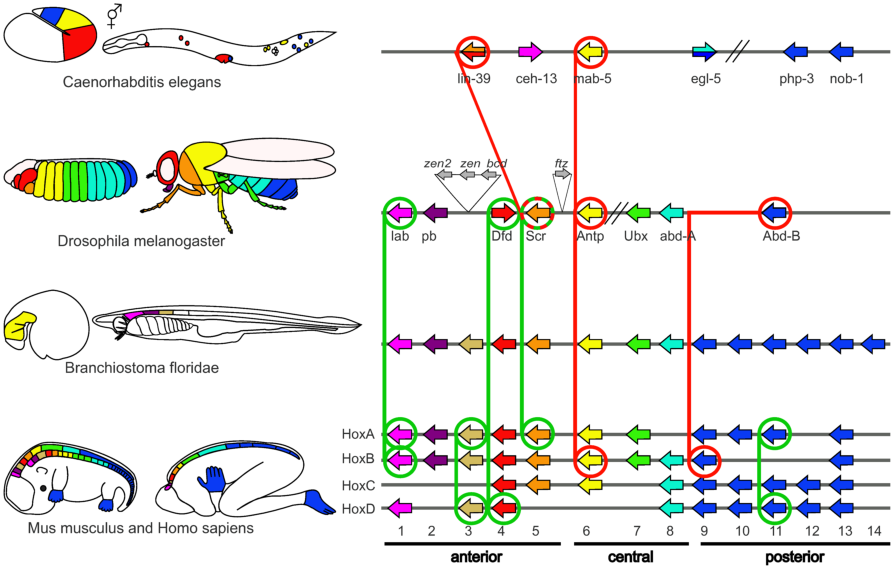
\includegraphics[width=1\textwidth]{Figures/Intro/hox_colinearity.pdf}
\caption[Hox colinearity]{ Expression pattern of Hox genes and genomic structure of Hox clusters in different phyla represented by model organisms, illustrating the concept of collinearity. The Hox genes are classified according to their expression pattern. Modified from \parencite{hueber_improving_2010}
}
\label{fig:Intro_hox_colinear}
\end{figure} 

\section{The vertebrate body plan}


The vertebrate body plan is one of the most successful in the tree of life. It has allowed these animals to adapt to a very wide range of ambient conditions. Vertebrates have two sister phyla, cephalochordates and tunicates. Together, these three lineages of animals conform to what we know as chordates. The body plans of vertebrates, cephalochordates and tunicates have evolved from the ancestral chordate one. Comprehending the ancestral chordate body plan is essential to understand the innovations that vertebrates have incorporated on top of it.
One of the main characteristics of chordates is the presence of an anatomical structure called notochord \parencite{stemple_structure_2005, bree_development_2018}. The notochord is a rod-shaped structure that appears after the gastrulation of the chordate embryos along the anteroposterior (AP) axis of the embryo. The notochord is a key developmental tissue which produces morphogens that control the axis specification of chordate embryos. Importantly, the GRN that determines how chordate embryos gastrulate and form the notochord is conserved across all chordates \parencite{di_gregorio_chapter_2020}. Another characteristic of this animal group is the presence of a hollow neural tube, which is dorsal to the notochord. This neural tube will give rise to the adult nervous system. The formation of this tube is known as neurulation, during which the neural plate borders elevate and fuse at the dorsal midline, the "crest" of the neural tube \parencite{nikolopoulou_neural_2017, moon_mechanics_2022}. This mechanism is conserved along all chordate lineages. Of the three groups of animals that make up chordates, cephalochordates are the most similar living group to the common chordate ancestor, due to their low evolutionary rate \parencite{delsuc_tunicates_2006}. That is why researchers have used an animal belonging to this group in order to understand better the development of chordates. This animal is amphioxus (\textit{Branchiostoma sp.}), a small fish-shaped organism that lives in shallow waters worldwide and has been extensively used in developmental studies in order to understand the novelties of vertebrate body plan over the chordate one \parencite{putnam_amphioxus_2008, acemel_single_2016,escriva_my_2018, marletaz_amphioxus_2018, aldea_genetic_2019, meister_functions_2022}.

On top of the chordate body plan, the vertebrate lineage has developed several novelties that separate them from other chordates. The most defining novelty is the presence of a backbone and an endoskeleton. Within vertebrates, we can distinguish two groups, gnathostomes and cyclostomes. In gnathostomes, we can find another vertebrate morphological novelty, the appearance of paired appendages, such as limbs and fins \parencite{freitas_new_2014, cass_conserved_2021}. These paired appendages have played a crucial role in the adaptation and diversification of many species. Paired appendages allow for movement and manipulation of the environment, enabling vertebrates to move on land, climb trees, or swim in the water, which created new niches to thrive in and led to the diversification of many lineages. The presence of paired appendages and the formation of a jaw is what separates gnathostomes from cyclostomes. In both vertebrate groups, we find another vertebrate novelty over the chordate body plan, the specified head, which typically contains paired sensory organs like ears and eyes. There is a clear relationship between the emergence of these new structures and the appearance of a vertebrate-specific cell type, the neural crest cells \parencite{york_evolutionary_2020, martik_riding_2021, rothstein_evolutionary_2023}. These cells have their developmental origin at the end of neurulation when the "crests" of the neural tube have fused. When the neurulation is complete, these cells migrate to different parts of the head and trunk of the embryo. These migrated neural crest cells will give rise to several tissues and structures, like the aforesaid cranial endoskeleton, heart primordium, and melanocytes among many others. Of special interest are also the sensory placodes that are located in the head of the developing vertebrates. These placodes interact with the neural crest cells and give rise to the paired sensory organs that characterize the head of vertebrates. Another characteristic of the specialised head of vertebrates is the presence of specific muscles that allow vertebrates to perform several functions with the head, from chewing to facial expressions. How these novelties have arisen in vertebrates over the chordate body plan has been a question that has puzzled researchers for years. In order to answer this question, research groups, including ourselves, have looked into how the regulatory information of the genome changes from chordates to vertebrates \parencite{van_otterloo_gene_2013, marletaz_amphioxus_2018}.



\section{Gene regulation as a source of phenotypic variation}


Most genes are shared and conserved up to a certain point in the animal kingdom. This implies that the morphological diversity of animals and how it has emerged relies upon the differential use of the same components \parencite{duboule_evolution_1998}. Gene regulation provides the means to deploy different genetic components in diverse situations and, thus, is one of the main drivers of evolution. A great example is the aforementioned Hox genes since they are conserved in the animal tree of life. Still, their differential deployment in different body segments leads to body plan diversity \parencite{mallo_reassessing_2018, turetzek_hox_2022}. Following the example of Hox genes, there are several cases in which changes in gene regulation lead to morphological novelties, like the formation of the snake body plan. In tetrapods, the vertebrate lineage to which snakes belong, the ribs only develop at the thoracic segment of the trunk, and the expression of \textit{Hoxa10} in the abdominal part of the trunk inhibits their formation \parencite{wellik_hox10_2003}. This is not the case in snakes, where ribs develop in both thoracic and abdominal parts of the trunk, even in the part where \textit{Hoxa10} is expressed \parencite{woltering_axial_2009}. This is not due to the loss of function of snake \textit{Hoxa10} since its expression in mice leads to the inhibition of rib development \parencite{guerreiro_role_2013}. Taking into account the several functions that this gene plays during development, a total loss of function would be deleterious. In contrast, it has been shown that the presence of a mutation in an enhancer to which \textit{Hoxa10} binds is responsible for this regionalized loss of rib-repressive function in these animals \parencite{guerreiro_role_2013}. This mutation was also found in another taxon of animals, the mammalian Paenungulata taxon which includes elephants and manatees, which also presents an expansion of the ribcage, demonstrating how changes in the regulatory information of key developmental genes can lead to novel traits. Another example of how evolution has tampered with the regulatory information encoded in enhancers is the case of limbless snakes \parencite{leal_loss_2016, kvon_progressive_2016, leal_developmental_2018}. The ZRS, a unique limb enhancer, controls Shh expression in limb buds of developing embryos. Its removal leads to a phenotype that resembles an \textit{Shh} loss of function phenotype, but only on the limbs \parencite{sagai_elimination_2005}. In snakes, the ZRS sequence is degenerated and leads to the abolishment of Shh expression in limbs and stalling of the development of these structures. These examples illustrate the importance of understanding the evolutionary implications of changes in gene regulation.


Another source of change leading to morphological novelties of vertebrate body plan are genome duplications. In vertebrates, the gnathostome lineage has undergone two rounds of whole genome duplication (WGD) \parencite{dehal_two_2005, putnam_amphioxus_2008}. This means one gene in the ancestral chordate can have up to four copies in gnathostome lineages. Furthermore, teleost fishes have undergone an additional round of WGD \parencite{taylor_genome_2003, braasch_spotted_2016, simakov_deeply_2020}. These WGD events have a great influence on evolution since they increase the possibilities of variations in developmental gene expression without affecting fitness. A gene in the chordate ancestor would have up to four copies in vertebrates or eight in the case of teleosts, and these copies are named ohnologs \parencite{ohno_evolution_1970}. The presence of these ohnologs in the vertebrate's genomes makes it possible for these genes to diverge in their functions. To understand deeper the regulatory changes that have contributed to evolutionary novelties, studies based on comparative genomics are broadly used, facilitated by the recent sequencing of numerous animal genomes. As an example of this kind of studies, we have previously used amphioxus as a proxy for the chordate ancestor since it does not have undergone any of these vertebrate-specific WGD \parencite{marletaz_amphioxus_2018}, and compared it with a teleost that suffered three rounds of WGD, the zebrafish. For those genes retained in a 1-to-1 ortholog, we found that the expression domain tends to be the same in zebrafish than in amphioxus, retaining the ancestral expression pattern. In contrast, if we analyse the expression pattern of zebrafish ohnologues (1-to-many copies retained), we find that each ohnologue copy shows a different expression pattern compared to the ancestral. Generally, expression patterns of zebrafish ohnologs complement each other, and the aggregated expression of all of them resembles the ancestral one (Figure \ref{fig:Intro_ohnologs}). Genes implicated in embryonic development and transcriptional regulation, like TFs, tend to retain more copies in vertebrates. Usually, at least one of the ohnologs has a larger regulatory landscape and is populated with more enhancers. Three different situations can be observed among the expression domains of the ohnologue genes in zebrafish: redundancy, subfunctionalization and specialization. In the first case, redundancy, the ohnolog retains the same expression pattern as the ancestral gene. Subfunctionalization implies the loss of some expression domains in the ohnologue gene compared to the ancestral one. In the case of specialization, the ohnologue loses all ancestral expression domains but one. In the majority of the ohnologue families, at least one gene has undergone specialization, and this process is associated with a gain of regulatory information. These genes tend to gain CREs in their regulatory landscape in vertebrates, enabling a more tight gene regulation. This gain of regulatory information after WGD in key developmental genes has probably contributed to the evolution of morphological novelties in vertebrates. There are other examples of WGD that have contributed to the evolution of specific lineages of gnathostomes, like the WGD duplication that we find in the tetrapod \textit{Xenopus laevis}. This frog has undergone an extra round of WGD, which is more recent than the gnathostome WGDs. The ease of study of the embryonic material of these frogs has led researchers to use it as model organism in order to understand the early effects of WGD in gene regulation \parencite{elurbe_regulatory_2017}. Elurbe and colleagues found that one copy of the duplicated genome tends to degenerate faster than another, and these mechanisms of degeneration and rearrangement depend on transposable elements. In general, WGDs allow the diversification and specialization of gene repertoires in animals due to the diversification of gene fate and the increase of the regulatory complexity of these genes.


\begin{figure}[ht]
\centering
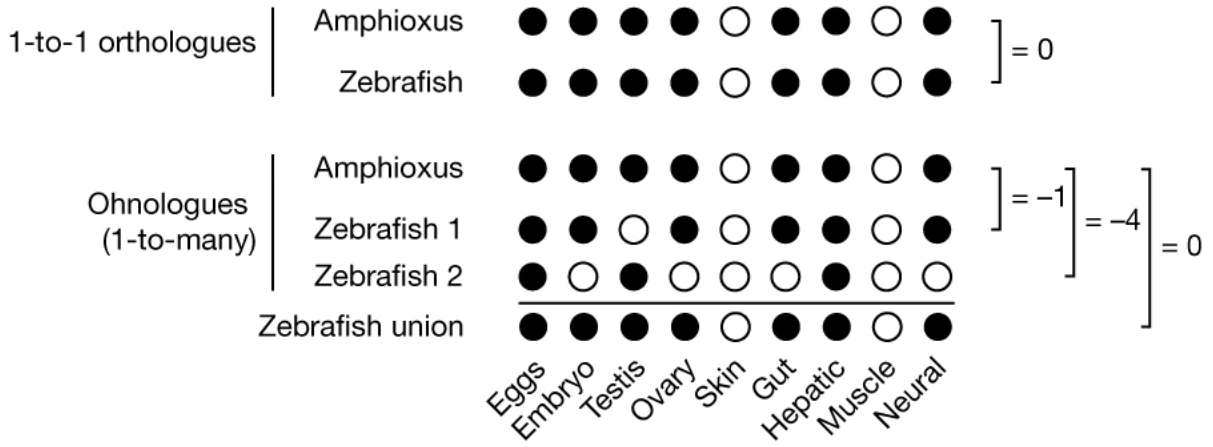
\includegraphics[width=1\textwidth]{Figures/Intro/Ohnologs_expression.png}
\caption[Ohnologs expression]{Schematic representation of how ohnologs retain the ancient gene expression. In the case of genes for which only one vertebrate copy was retained, called here 1-to-1 orthologues, the expression pattern domains are very similar. In genes whose copies are retained, the expression pattern of the ohnologs may vary regarding the ancient gene, but the sum of their expression domains resembles the ancient gene expression pattern. Modified from \parencite{marletaz_amphioxus_2018}.
}
\label{fig:Intro_ohnologs}
\end{figure} 


As previously described, GRNs are important for initiating transcriptomic programs during development. Changes in these GRNs themselves can lead to phenotypic variation and the evolution of new traits, like the case of the snake body plan. Changes in regulatory regions can lead to the deployment of an existing GRN in a completely novel tissue and transcriptomic context. This phenomenon is known as GRN co-option \parencite{mcqueen_chapter_2020}. There are several examples of this phenomenon in vertebrate evolution. An interesting example of this is the co-option of the unpaired fin developmental GRN to form the paired fins \parencite{letelier_conserved_2018}. In this work, Letelier and colleagues trace the evolutionary history of the ZRS enhancer in vertebrates using medaka (\textit{Oryzias latipes}) as an animal model. Similarly to the findings of the studies in snakes \parencite{leal_loss_2016, kvon_progressive_2016}, tinkering with the ZRS enhancer leads to defects in paired appendages development. Interestingly, the development of the dorsal fin was also impaired by the deletion of this enhancer. Since the emergence of this unpaired largely predates the appearance of the paired appendages, this suggests that this developmental program existed first in unpaired appendages and was co-opted in paired appendage development. This example showcases how GRN co-option can lead to a gain of pleiotropy. 
GRN co-option has also occurred outside the vertebrate tree. Murugesan and colleagues \parencite{murugesan_butterfly_2022}, using different genomics analyses and tools, have found that the eyespots of butterflies have a transcriptomic profile similar to that of the antennae. This implies that the GRN driving antennae development has also been deployed in a different developmental tissue, the wings, which enabled the emergence of a novel trait as the eyespots. Moreover, when mutating the CREs that control the expression of key genes in the GRN, both antennae and eyespots are lost in the embryo. This example pinpoints how GRN co-option has been used widely in the tree of life so that new traits evolve. 
All the examples examined here and in previous sections occur in a relatively large amount of time, but evolution and its mechanisms can also operate in short periods of time, thanks to the fine-tuning of gene regulation.




\section{The role of gene regulation at microevolutionary scales}

In previous chapters, we have described several examples demonstrating the relationship between gene regulation and evolution. The example of WGD in \textit{Xenopus laevis}, previously described, shows how evolutionary mechanisms can operate in shorter scales of time \parencite{elurbe_regulatory_2017}. Gene regulation and evolution can operate at even shorter scales of time, for example, when adaptation to a new environment occurs. During the adaptation to a new environment, several processes can make it possible for a certain population to adapt. We have to consider that in these cases, we may not be able to separate evolution, understood as the selection of traits during generations that make the population fitter to the new environment, from other processes like phenotypic plasticity or metabolic swifts in the individuals. In any case, the regulation of the genome plays an important role in the adaptation to new environments, regardless if this process takes place during hundreds of generations or if it is during a few of them. This is the case of stickleback, which has colonized significantly disparate environments, from freshwater rivers and lakes to marine environments \parencite{reid_threespine_2021}. The stickleback populations in each habitat possess underlying genomic variations. Upon natural selection, the individuals with the genetic background that makes them thrive in each environment are positively selected. These adaptations to a new environment occur over decades and in parallel in different locations. When examining variations in the genome, it was found that they were mainly regulatory regions that affect key genes for adaptation to freshwater or salty water environments, like the ones that control the length of dorsal and pelvic spines, the number of armour plates, etc. \parencite{jones_genomic_2012, roberts_kingman_predicting_2021, bassham_repeated_2018}. Stickleback is a great model organism in order to understand parallel evolution and the effect of standing genomic variation in the adaption to a new environment.

Similarly, \textit{Astyanax mexicanus}, also known as the Mexican tetra or blind cavefish, constitutes a great model species to investigate adaptation to a new environment. The surface-dwelling and cave-dwelling populations of this species provide a unique opportunity to study how evolution shapes the development and genetic makeup of organisms in response to different environments (Figure \ref{fig:Intro_cavefish}). Cavefish are particularly interesting to study because they can provide a glimpse into the processes of adaptation and speciation. In comparison to the surface-dwelling, the cave-dwelling populations of \textit{Astyanax mexicanus} have lost their eyes and pigmentation and developed enhanced sensory capabilities, such as improved lateral line and smell systems, in response to the dark and stagnant conditions of their underground habitats \parencite{jeffery_emerging_2008, jeffery_astyanax_2020}. Moreover, they have an altered metabolism due to the food disponibility in caves, making them a good model for understanding metabolic diseases \parencite{rohner_cavefish_2018, krishnan_sweet_2019}. More strikingly, these adaptations have occurred in a very short period of time, from 20.000 to 200.000 years ago \parencite{fumey_evidence_2018, herman_role_2018}, and the phenotypes have evolved in parallel in independent cavefish populations \parencite{niven_evolution_2008}. The study of the genetic basis of adaptation of Astyanax is possible since the genomes of the different populations have already been sequenced \parencite{warren_chromosome-level_2021}. Importantly, there are several tools for genetic edition adapted to this model organism  \parencite{ma_genome_2015, klaassen_crispr_2018, stahl_manipulation_2019}, allowing for precise genetic manipulations in \textit{Astyanax mexicanus}.  Additionally, the use of genome-wide approaches, such as transcriptomics and genomics, makes it feasible to understand how genetic changes have shaped the adaptation of this species to cave environments \parencite{stahl_manipulation_2019, oliva_characterizing_2022}.

\begin{figure}[ht]
\centering
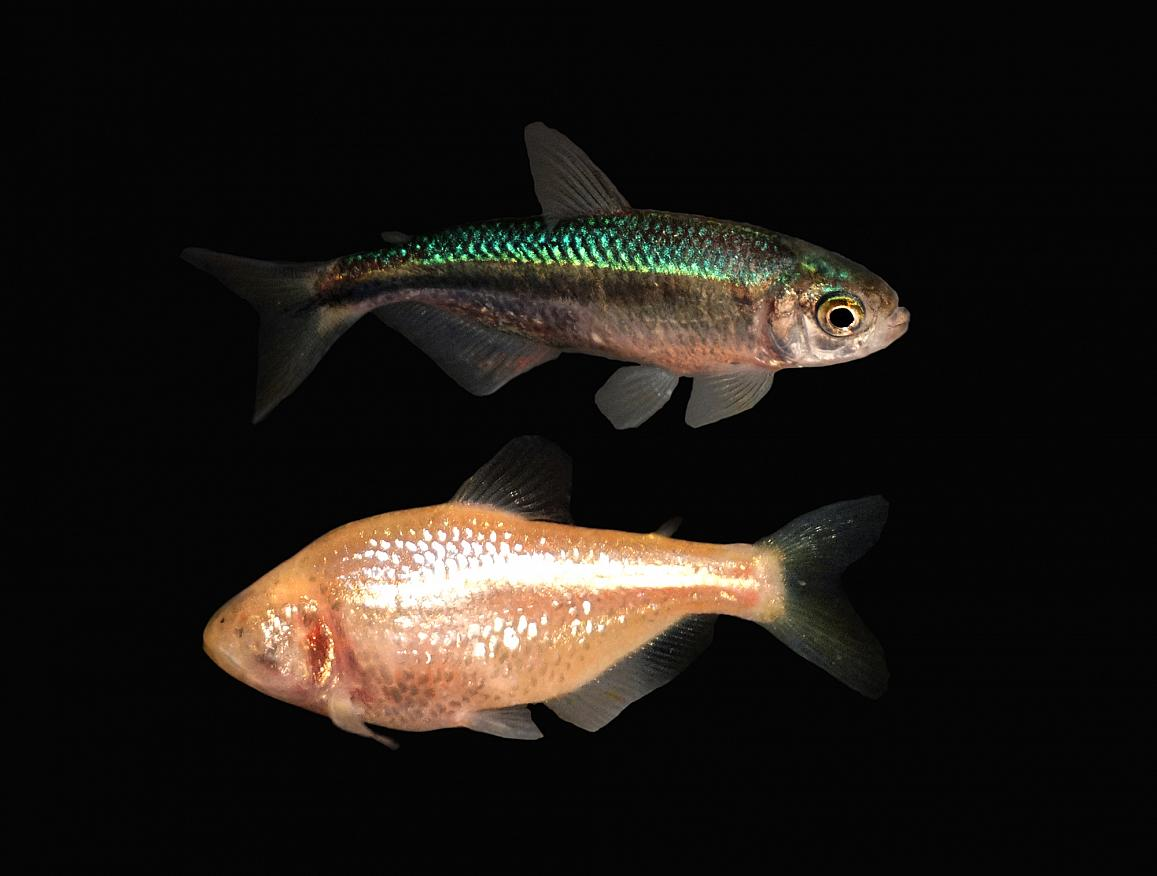
\includegraphics[width=1\textwidth]{Figures/Intro/Intro_cavefish.jpg}
\caption[Comparison of populations of \textit{Astyanax mexicanus}]{Comparison of surface-dwelling (top) and cave-dwelling (bottom) populations of \textit{Astyanax mexicanus}. The latter is native to Pachón cave. Animals from this population have completely lost their eyes and pigmentation due to the adaptation to the cave environment. The \textit{Pachón} population of cavefish is one of the most studied in genomics studies. Credit: Daniel Castranova, NICHD/NIH
}
\label{fig:Intro_cavefish}
\end{figure} 

In order to better understand the processes that have driven the fast adaptation of cavefish to the new environment, researchers have bred Surface dwelling individuals in the dark \parencite{bilandzija_phenotypic_2020} during one generation. Those surfacefish bred in dark conditions showed some phenotypic characteristics that resembled the ones present in cavefish individuals affecting morphology and metabolism. For instance, the offspring of surfacefish raised in dark conditions, the second generation, showed a decreased metabolic rate, which resembles the metabolic rate of cavefish. Moreover, dark-raised individuals are more resistant to starvation due to their lower metabolic rate and tend to accumulate more fat in their bodies, just like cavefishes. Furthermore, they present increased levels of cortisol along with other hormonal changes. This phenotypic plasticity would partially explain the quick adaptation to the cave environment of \textit{Astyanax mexicanus}. An important question arose then: Can the plastic changes observed be inherited in the next generation? To test this, Bilandžija and colleagues compared the offspring of dark-raised and light-raised animals by rearing them in different conditions, complete darkness or normal light-dark cycles. When larvae were put in light conditions, they did not show any differential phenotype between them, independently of their progenitor's origin. For example, the F1 grown on light-dark cycles showed the same resistance to starvation, even if the progenitors were raised in different conditions. On the other hand, larvae exposed to constant dark increased resistance to starvation, compared to larvae raised in light-dark cycles. In the case of the F1 of dark-raised individuals, they showed a slight improvement in this starvation survival compared to the offspring of light-raised individuals. These results suggest that these plastic changes can be refined in successive generations, and this implies that plasticity itself is genetically determined and thus can be inherited. The influence of phenotypic plasticity in evolution and the evolvability of this plasticity is still under debate in the scientific community \parencite{fox_beyond_2019, kristensen_adaptation_2020, mallard_evolution_2020}. Some studies have already used cavefish to understand the role of developmental and phenotypical plasticity in cave adaptation \parencite{bilandzija_phenotypic_2020, blin_developmental_2018}. The use of other cavefish species' adaptation to the new environment will help to discern between general mechanisms of adaptation and species-specific mechanisms \parencite{behrmann-godel_phenotypic_2023}. Overall, \textit{Astyanax mexicanus} is a great model to unravel the role of gene regulation at the microevolutionary scale and also determine which is the impact of phenotypic plasticity on it.












